% hello.tex - Our first LaTeX example!

\documentclass{article}
\usepackage[dvipsnames]{xcolor}
\usepackage{pgf,tikz,pgfplots,graphicx}
\usepackage{wrapfig}
\usepackage{lipsum}
\usepackage{amsmath,amsfonts}
\pgfplotsset{compat=1.3}
\usepackage{mathrsfs}
\usepackage{mathtools}
\usepackage{caption}
\usepackage{subcaption}
\newcommand{\redbox}[1]{%
     \fcolorbox{red}{white}{
     \parbox{\textwidth}{%
        #1
    }%
    }
}
\newcommand\reddashedbox[1]{
\tikz [baseline=(boxed word.base)] \node (boxed word) [draw=red, rectangle, dashed, line cap=round] {#1};
}
\newcommand{\exampleblue}[1]{
    \textcolor{RoyalBlue}{#1}
}
\newcommand*\theoremsquare[1]{\tikz[baseline=(char.base)]{
            \node[shape=rectangle,draw,inner sep=2pt] (char) {\footnotesize #1};}}
\usetikzlibrary{arrows}

\begin{document}

\title{Calculus Notes}
\author{Jack Gong\\
Pinetree Secondary\\
  \texttt{haotiangong@hotmail.com}}
\date{\today}
\maketitle
\newpage
\tableofcontents
\newpage



\section{Intro}
\newpage

\section{Limits}
\subsection{Ideas about limits}

\medskip
We write $$\lim_{x\rightarrow a}f(x)=L$$ \begin{center}
  and say the limit of f(x) as x approaches a is L
  \end{center}

\bigskip
\redbox{

  \textcolor{red}{\theoremsquare{1}} $$ \lim_{x\rightarrow a}f(x)=L$$ if and only if
  \begin{itemize}
  \item $\lim_{x\rightarrow a^-}f(x)=L$
  \item $\lim_{x\rightarrow a^+}f(x)=L$
  \end{itemize}

}



\begin{figure}[h]
\centering
\begin{subfigure}{.5\textwidth}
  \centering
  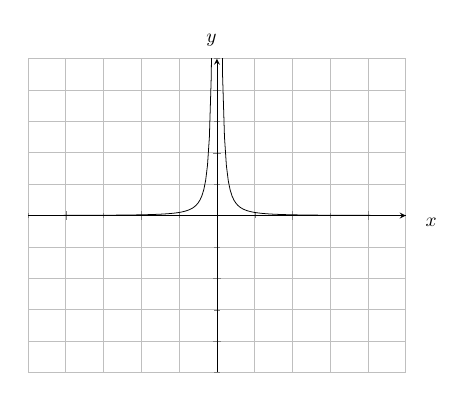
\begin{tikzpicture}[scale = 0.7]

  \begin{axis}[grid=both,ymin=-50,ymax=50,xmax=5,xmin=-5,xticklabel=\empty,yticklabel=\empty,
                 minor tick num=1,axis lines = middle,xlabel=$x$,ylabel=$y$,label style =
                 {at={(ticklabel cs:1.1)}}]
  \addplot[domain = -5:5, samples = 201, color = black]
  {1/x^2};
  \end{axis}
  \end{tikzpicture}
  \caption{$y=\frac{1}{x^2}$}
\end{subfigure}%
\begin{subfigure}{.5\textwidth}
  \centering
  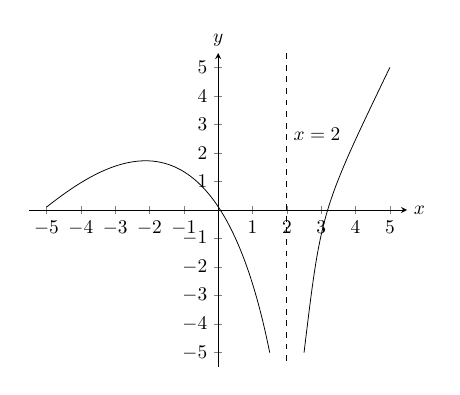
\begin{tikzpicture}[scale = 0.7]
  \begin{axis}[
    axis x line=center,
    axis y line=center,
    xtick={-5,-4,...,5},
    ytick={-5,-4,...,5},
    xlabel={$x$},
    ylabel={$y$},
    xlabel style={at={(1,0.5)},right},
    ylabel style={at={(0.5,1)},above},
    xmin=-5.5,
    xmax=5.5,
    ymin=-5.5,
    ymax=5.5]
    \draw[dashed] (axis cs:2,5.5) -- node[pos=0.3, anchor = south west]{$x=2$}(axis cs:2,-5.5);
    \draw(axis cs:-5,0.1) .. controls(axis cs:-3,2) and (axis cs:0,4) .. (axis cs:1.5,-5);
    \draw(axis cs:2.5,-5) .. controls(axis cs:3,0) .. (axis cs:5,5);
    \end{axis}
    \end{tikzpicture}
  \caption{$y$ approaches $-\infty$  as \newline x approaches 2}
\end{subfigure}
\end{figure}

As seen in figure a) and b), both functions have a limit approaching infinity. We write their limits as $$\lim_{x\rightarrow a}f(x)=(\pm)\infty$$
Thus, we say $x=a$ are their \textbf{asymtotes}.

\subsection{Finding Limits}
\noindent \exampleblue{\textit{Example 1.} Show that $\lim_{x\rightarrow 0}|x| = 0 $} \newline

\[
    |x|=
\begin{cases}
    x,            & \text{if } x\geq 0\\
    -x,           & \text{if } x< 0
\end{cases}
\]

By analysis, $$\lim_{x\rightarrow 0^+}|x|  = \lim_{x\rightarrow 0^+} x = 0$$
$$\lim_{x\rightarrow 0^-}|x|  = \lim_{x\rightarrow 0^-} x = 0$$

By theorem 1, $$\lim_{x\rightarrow 0^-}|x| = \lim_{x\rightarrow 0^+} |x|$$
$$\Downarrow$$
$$\lim_{x\rightarrow 0} |x| = 0$$

\noindent \exampleblue{\textit{Example 2.} Find $\lim_{x\rightarrow3^+} \frac{2x}{x-3}$ and $\lim_{x\rightarrow3^-} \frac{2x}{x-3}$ }

\bigskip
By analysis, if $x$ approaches 3 from the right side, then $(x+3)$ is a small positive integer, then $(x+3)$ is a really small pos. integer; the result is a large pos. int.\par

If $x$ approaches 3 from the left side, then $(x+3)$ is a small neg. integer. The result is a large neg. int.

$$\lim_{x\rightarrow 3^+} \frac{2x}{x-3} = \infty$$
$$\lim_{x\rightarrow 3^-} \frac{2x}{x-3} = -\infty$$

\begin{center}
\begin{figure}[h]
  \centering
  \begin{tikzpicture}[scale = 1.0]
  \begin{axis}[
    axis x line=center,
    axis y line=center,
    xlabel={$x$},
    ylabel={$y$},
    xlabel style={at={(1,0.5)},right},
    ylabel style={at={(0.5,1)},above},
    xmin=-10.5,
    xmax=10.5,
    ymin=-10.5,
    ymax=10.5]
    \draw[dashed] (axis cs:3,10.5) -- node[pos=0.3, anchor = south west]{$x=3$}(axis cs:3,-10.5);
    \addplot[domain = -10:10, samples = 201, color = black]
    {2*x/(x-3)};
    \end{axis}
    \end{tikzpicture}
\end{figure}
\reddashedbox{However, the lim is still non-existant.}
\end{center}

\newpage

\noindent \exampleblue{\textit{Example 3.} Limit of $y=tan(x)$ }

\begin{center}
\begin{figure}[h]
  \centering
  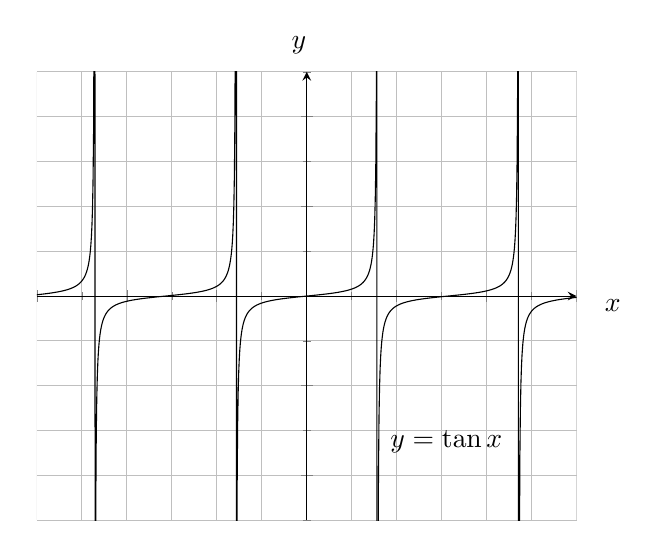
\begin{tikzpicture}[scale = 1.0]
  \begin{axis}[grid=both,ymin=-50,ymax=50,xmax=6,xmin=-6,xticklabel=\empty,yticklabel=\empty,
                 minor tick num=1,axis lines = middle,xlabel=$x$,ylabel=$y$,label style =
                 {at={(ticklabel cs:1.1)}}]
  \addplot[domain = -6:6, samples = 1001, color = black]
  {tan(deg(x))};
  \end{axis}
    \node at(5.2, 1) {$y=\tan x$};
  \end{tikzpicture}
\end{figure}
\end{center}

The vertical asymtotes are:

$$ x = \frac{\pi}{2} + n\pi \:(n\in \mathbb{Z}) $$

\subsection{Asymtotes}
When at least one of the following is true: \newline
$$\lim_{x\rightarrow a}f(x)=\infty,    \lim_{x\rightarrow a^-}f(x)= \infty,   \lim_{x\rightarrow a^+}f(x)= \infty, $$ \newline

$$\lim_{x\rightarrow a}f(x)=-\infty,   \lim_{x\rightarrow a^-}f(x)= -\infty,  \lim_{x\rightarrow a^+}f(x)= -\infty, $$


\redbox{\medskip \centering $x=a$ is a vertical asymtote. \medskip}
\newpage

\subsection{Limit Laws}
*Suppose $c$ is a constant and $\lim_{x\rightarrow a} f(x)$ and $\lim_{x\rightarrow a} g(x)$ exists,
\medskip

\redbox{
\begin{spreadlines}{20pt}
\begin{gather}
\lim_{x\rightarrow a} [f(x)+g(x)] = \lim_{x\rightarrow a} f(x) + \lim_{x\rightarrow a} g(x) \\
\lim_{x\rightarrow a} [f(x)-g(x)] = \lim_{x\rightarrow a} f(x) - \lim_{x\rightarrow a} g(x) \\
\lim_{x\rightarrow a} [cf(x)] = c\lim_{x\rightarrow a} f(x)\\
\lim_{x\rightarrow a} [f(x)g(x)] = \lim_{x\rightarrow a} f(x) \cdot \lim_{x\rightarrow a} g(x) \\
\lim_{x\rightarrow a} \frac{[f(x)]}{[g(x)]} = \frac{\lim_{x\rightarrow a} f(x)} {\lim_{x\rightarrow a} g(x)}  \:(\lim_{x\rightarrow a} g(x)\neq 0)
\end{gather}
\end{spreadlines}}

\redbox{
  \centering
  $$\lim_{x\rightarrow a} [f(x)]^n = [\lim_{x\rightarrow a}f(x)]^n$$ \newline
  $$\lim_{x\rightarrow a} \sqrt[n]{f(x)} = \sqrt[n]{\lim_{x\rightarrow a} f(x)}$$
}

\subsection{Limit Calculations}
\noindent\exampleblue{\textit{Example 1.}
       Find $\lim_{h\rightarrow 0} \frac{(3+h)^2-9}{h}$
}

\begin{align*}
  F(h) &= \frac{(3+h)^2-9}{h}\\
       &= \frac{h^2+6h+9-9}{h}\\
       &= h+6
\end{align*}
By evaluation, $\lim_{h\rightarrow 0} h+6 = 6$
\newpage

\subsubsection{Direct Substitution Property}

\hspace{1cm} If $f$ is a \textbf{polynomial} or a \textbf{rational function} and $a$ is in the domain of $f$, then:\newline
\redbox{\centering $$\lim_{x\rightarrow a} f(x) = f(a)$$}
\medskip

\noindent\exampleblue{\textit{Example 2.}
       Find $\lim_{t\rightarrow 0} \frac{\sqrt{t^2+9}-3}{t^2}$
}

\begin{align*}
       &= \lim_{t\rightarrow 0} \frac{\sqrt{t^2+9}-3}{t^2} \cdot \frac{\sqrt{t^2+9}+3}{\sqrt{t^2+9}+3}\\
       &= \lim_{t\rightarrow 0} \frac{t^2+9-9}{t^2(\sqrt{t^2+9}+3)}\\
       &= \lim_{t\rightarrow 0} \frac{t^2}{t^2\sqrt{t^2+9}+3t^2}\\
       &= \lim_{t\rightarrow 0} \frac{1}{\sqrt{t^2+9}+3}\\
       &= \frac{1}{\sqrt{\lim_{t\rightarrow 0} t^2 +9} +3}\\
       & = \frac{1}{\sqrt{9}+3} = \frac{1}{6}
\end{align*}

\noindent\exampleblue{\textit{Example 3.}
       Find $\lim_{x\rightarrow 1} \frac{\sqrt[3]{x}-1}{\sqrt{x}-1}$
}

\end{document}
